\documentclass[class=book, crop=false]{standalone}
\usepackage[utf8]{inputenc}
\usepackage[subpreambles=true]{standalone}
\usepackage{import}
\usepackage{amsmath}
\usepackage{amssymb}
\usepackage[margin=1.2in]{geometry}
\usepackage[sorting = none,
            doi = true  %lesedato for url-adresse
            ]{biblatex} %none gir bibliografi i sitert rekkefølge
\addbibresource{reference.bib}
\usepackage{csquotes}

%\usepackage{float}

\begin{document}



%\chapter{Electrical power system}
The reinforcement agent is working within an electrical power system and it is therefore necessary to give an introduction to the electrical grid and relevant quantities describing it. 

\section{Electric circuit theory}
\subsection{Voltage, current and power}
An electric circuit is a model that describes how electrical power is transferred from a electrical source unit to a load. An example of a source is a power socket on the wall and a load can be a light bulb or a vacuum cleaner. A model of a simple electric circuit is shown in figure \ref{fig:theory:simple_circuit}, where \textit{U} is placed next to the electrical source and \textit{R} next to the load. The electric transmission system is analogous to this configuration, except it with several electrical sources (power plants) and loads (cities) connected. 

\begin{figure}[ht!]
    \centering
    \subimport{../}{circuits/simple_circuit.tex}
    \caption{Simple electric circuit with voltage source \textit{U}, current \textit{I} and resistance \textit{R}.}
    \label{fig:theory:simple_circuit}
\end{figure}



\textit{U} is the voltage in the circuit and is a measure of the potential energy between charges at each end of the voltage source. Volt (V) is the unit for voltage, which is equivalent to joule per coulomb. The current \textit{I} flowing in the wire is a measure for the amount of charges passing through a cross section of the circuit wire per second. The unit for current is ampere (A) or coulomb per second. The resistance \textit{R} is a measure for how much an electric load, such as a light bulb, resists the flow of electric charges. The unit for resistance is ohm, denoted by $\Omega$. The magnitudes of the voltage, current and resistance are governed by Ohm's law

\begin{equation}\label{eq:theory:ohm_simple}
    U = RI
\end{equation}

where  \textit{U} is the voltage, \textit{R} is the resistance and \textit{I} is the current flowing. Another version of this is equation is found by introducing the admittance $Y$ which is defined as the inverse of the resistance $R$, i.e  $Y = 1/R$. The admittance $Y$ is a measure for how a load allows the flow charges in a circuit. The unit for admittance is siemens (S). By using the admittance $Y$, Ohm's law can be expressed as
\begin{equation}\label{eq:theory:ohm_simple_inverse}
    I = UY
\end{equation}

The power $P$ an electric load consumes can be found easily by multiplying the current \textit{I} and voltage drop \textit{U} over the load
\begin{equation}\label{eq:theory:apparent_power}
    P = UI
\end{equation}
The unit for power is watt (W) or joule per second.

\subsection{Kirchoff's laws}
Figure \ref{fig:theory:simple_circuit_branches} shows a circuit with several branches and loads 

\begin{figure}[ht!]
    \centering
    \subimport{../}{circuits/simple_circuit_branches.tex}
    \caption{Simple electric circuit with several branches and resistors}
    \label{fig:theory:simple_circuit_branches}
\end{figure}

The current \textit{I} will split when it reaches and intersection, in such a way that the total current flowing into the node equal the total total current flowing out from a node. Referring to figure \ref{fig:theory:simple_circuit_branches} we have that $I = I_1 + I_2$. This conservation of current is called Kirchoff's 1st law or simply Kirchhoff current law (KCL). With the introduction of branches in a circuit, there will also be closed loops. In figure \ref{fig:theory:simple_circuit_branches} there are two closed loops $C_{1}$ and $C_{2}$. Kirchoff's 2nd law , aslo known as Kirchoffs's voltage law (KVL), states that the voltage \textit{U} over the components in a closed loop $C$ is equal to zero. 

\begin{equation}\label{eq:theory:kirchoffs_2nd_integral}
    \sum_{i}^{N} V_{i} = 0, \;\; V_{i} \in C
\end{equation}
For the two loops $C_1,C_2$ in figure \ref{fig:theory:simple_circuit_branches} we have 


\begin{equation}
   \begin{aligned}\label{eq:theory:krirchoffs_2nd_ex}
    U + I_{1}R_{1} = 0 
    \\
    I_{1}R_{1} - I_{2}R_{2} = 0
\end{aligned} 
\end{equation}

\section{Reactive components}
There are electrical loads that cause a phase shift between the current and voltage in an electric circuit. For instance, the circuit shown in figure \ref{fig:theory:circuit_capacitor} has a capacitor as load.


\begin{figure}[ht!]
    \center
    \subimport{../}{circuits/circuit_capacitor.tex}
    \caption[size = 9]
    {Circuit with a capacitor as load}\label{fig:theory:circuit_capacitor}
\end{figure}



A capacitor is a component that can store an electrical charge \textit{Q} when a direct current (DC) voltage source \textit{U} is applied over it. A capacitor is characterised by how much charge \textit{Q} it can hold for a given DC voltage \textit{U}. This quantity is called the capacitance \textit{C} of the capacitor and is given by 

\begin{equation}
   \begin{aligned}\label{eq:theory:capacitance}
C = \frac{Q}{U}
\end{aligned} 
\end{equation}
where \textit{Q} is the charge stored by the capacitor and \textit{U} is the applied DC voltage. The units for capacitance is farad \textit{F}. Applying Kirchoff's voltage law to this circuit when the source is a sinusoidal signal $U\sin(\omega t)$ and using equation \eqref{eq:theory:capacitance} gives



\begin{equation}
   \begin{aligned}\label{eq:theory:capacitance_diffeq}
U\sin{(\omega t)} - \frac{Q(t)}{C} = 0, \;\;\; Q(0) = 0
\end{aligned} 
\end{equation}

Recognising that the current \textit{I} is the derivative of \textit{Q} with respect to time reveals that the the current is given as

\begin{equation}
   \begin{aligned}\label{eq:theory:capacitance_diffeq_solved}
I(t) = U\omega C \sin{(\omega t + \pi/2)}
\end{aligned} 
\end{equation}
The solution shows that the current \textit{I} is phase shifted 90 degrees ahead of the voltage \textit{U}. It is convenient to introduce the capacitive reactance $X_{c}$ as



\begin{equation}
   \begin{aligned}\label{eq:theory:reactance_capacitive}
X_{c} = \frac{1}{\omega C}
\end{aligned} 
\end{equation}
where $\omega$ is the angualar frequency of the signal and \textit{C} is the capacitance of the capacitor. The circuit current can now be expressed on the same form as Ohm's law

\begin{equation}
   \begin{aligned}\label{eq:theory:capacitance_diffeq_solved_ohm}
I(t) = \frac{U}{X_{c}} \sin(\omega t + \pi/2)
\end{aligned} 
\end{equation}

The circuit shown in figure \ref{fig:theory:circuit_inductor} is another example of a reactive component that phase shifts the current. 

\begin{figure}[ht!]
    \center
    \subimport{../}{circuits/circuit_inductor.tex}
    \caption[size = 9]
    {Circuit with a electromagnetic coil as load}\label{fig:theory:circuit_inductor}
\end{figure}

The load is an electromagnetic coil, also called an inductor, and appears in a wide range of electric components. For instance an electric transmission line is mainly modelled as an inductor. The voltage  across an electromagnetic coil is proportional to the derivative of the current flowing through it due to Faraday's law of induction. The proportional constant is called the inductance \textit{L} of the coil and it is given in henry \textit{H}. Similarly as with the capacitor, Kirchoff's voltage law  gives rise to a differential equation. Let the voltage source be $U\sin{(\omega t)}$

\begin{equation}
   \begin{aligned}\label{eq:theory:inductance_diffeq}
U\sin{(\omega t)} - LI'(t) = 0, \;\;\; I(0) = 0
\end{aligned} 
\end{equation}
The solution of equation \eqref{eq:theory:inductance_diffeq} is

\begin{equation}
   \begin{aligned}\label{eq:theory:inductancee_diffeq_solved}
I(t) = \frac{U}{\omega L}  \sin(\omega t - \pi/2)
\end{aligned} 
\end{equation}


The current is shifted 90 degrees behind the voltage in this case. We see that both inductors and capacitor shift the current by 90 degrees, but in different direction. The inductive reactance $X_{c}$ is defined as

\begin{equation}
   \begin{aligned}\label{eq:theory:reactance_inductive}
X_{c} = \omega L
\end{aligned} 
\end{equation}
where $\omega$ is the angular frequency of the voltage and $L$ is the inductance of the coil. 

\section{Reactive power}
For a purely resistive load with no phase shift between current and voltage, the instantaneous power transferred to the load as given by \eqref{eq:theory:apparent_power} is always positive, as shown in figure \ref{fig:theory:reactive_powers}. This power is called active power, and is measured in watt W. This is not the case for reactive loads. The phase shift between current and voltage results in a pulsating power between the source and the load, as shown in figure \ref{fig:theory:reactive_powers}. The pulsating power resulting from reactive loads is called reactive power \textit{Q} and has unit var, to distinguish it from unidirectional power flow. Figure \ref{fig:theory:reactive_powers} shows that the instantaneous power resulting from an inductive and capacitive load are opposite of each other. As a consequence, a circuit with equal inductive and capacitive reactance connected in parallel will draw zero instantaneous power from the source. By convention, a capacitive load is defined to supply reactive power while an inductive load is a reactive power consumer. Consequently, overhead transmission lines are considered reactive consumers, because they are mainly inductive. 

\begin{figure}[ht!]
    \center
    \subimport{../}{circuits/plot_powers.tex}
    \caption[size = 9]
    {Instantaneous power transferred to the load in a circuit with a pure resistive, inductive and capacitive load that are equal in size}\label{fig:theory:reactive_powers}
\end{figure}


\section{Voltage, current and power as complex numbers}

Current, voltage, impedance and and power are all expressed as complex numbers in an AC electric power system. Consider the circuit shown in figure \ref{fig:theory:complex_current_circuit}
\begin{figure}[ht!]
    \center
    \subimport{../}{circuits/complex_currents_circuit.tex}
    \caption[size = 9]
    {Circuit with a resistor and a inductance connected i parallel}\label{fig:theory:complex_current_circuit}
\end{figure}
The resistor will draw a current $I_{p}$ that is in phase with the source voltage. The inductor will draw a current $I_{q}$ that lags the voltage by 90 degrees. The resultant current drawn from the source will therefore be a linear combination of two phase shifted sinusoidal signals. The equations for summing phase-shifted sinusoidal signals are complicated, and not not easy to work with. Euler's formula states that a complex number $A$ can be expressed by

\begin{equation}\label{eq:eulers_equation}
    A = Re^{j\omega t} = R\cos{(\omega t)} + jR\sin{(\omega t)}
\end{equation}

where $e$ is the base of the natural logarithm, $j$ is the imaginary unit, $R$ is the magnitude of \textit{A}. The currents $I_{p}$ and $I_{q}$ signal can therefore be expressed as the imaginary part of two complex numbers $A_{1}, A_{2}$. Treating the currents as complex numbers makes it easier to sum them because they form a right angled triangle in the complex plane, as shown in figure \ref{fig:theory:phase_current}. One can always convert back to the sinusoidal current by taking the imaginary part of the complex resultant current \textit{I}.

\begin{figure}[ht!]
    \center
    \subimport{../}{circuits/phase_currents.tex}
    \caption[size = 9]
    {Current as complex numbers. $I_{q}$ is the current drawn by an inductor, and lags the voltage by 90 degrees. $I_{p}$ is the current drawn by a resistive load and is in phase with the voltage. The current \textit{I} is commonly defined to be lagging, so that $I = |I|e^{-j\varphi}$. By this definition, $\varphi$ is a positive real number when the current is lagging the voltage.   }\label{fig:theory:phase_current}
\end{figure}

The resultant current \textit{I} drawn from the voltage source can now be expressed as 
\begin{equation}
   \begin{aligned}\label{eq:theory:complex_current}
I = |I|e^{-j \varphi} = I_{p} + jI_{q}
\end{aligned} 
\end{equation}
where $|I|$ and $\varphi$ respectively are the magnitude and phase shift of the current. Comparing equation \eqref{eq:eulers_equation} and \eqref{eq:theory:complex_current} shows that the angular frequency $\omega$ is removed, and that the current is simply considered a complex constant. This has do with the fact that the sum of two synchronous sinusoidal signals inherits the same frequency. One can therefore simply consider the signal at t=0, and all calculations are correct. It is common to also express the complex current as $|I|\angle -\varphi$. The current magnitude $|I|$ is given by the Pythagorean theorem. 

\begin{equation}
   \begin{aligned}\label{eq:theory:pythagoras_current}
|I| = \sqrt{I_{p}^{2} + I_{q}^{2}}
\end{aligned} 
\end{equation}
The phase shift $\varphi$ is described by the trigonometric relation
\begin{equation}
   \begin{aligned}\label{eq:theory:phase_shift_current
   }
   \tan{\varphi} = -\frac{I_{q}}{I_{p}}
\end{aligned} 
\end{equation}



Inductive and capacitive reactances can also be expressed as complex numbers. A coil phase shifts the current 90 degrees behind the voltage. Considering the current $I_{q}$ as a complex number in Ohm's law gives that the inductive reactance can be expressed as $jX_{L}$, because multiplication by \textit{j} corresponds to a 90 degree rotation in the complex plane

\begin{equation}
   \begin{aligned}\label{eq:theory:complex_rectance_capacitive}
U = I\cdot jX_{L}
\end{aligned} 
\end{equation}

Similarly, a capacitive reactance $X_{c}$ phase shifts the current 90 degrees a head of the current. Therefore, it can be expressed as $-jX_{c}$

\begin{equation}
   \begin{aligned}\label{eq:theory:complex_rectance_inductance}
U = I\cdot (-jX_{c})
\end{aligned} 
\end{equation}

The complex notation also works for a circuit with resistive, inductive and capacitive components connected in series, as shown in figure \ref{fig:theory:complex_impedance_series}.

\begin{figure}[ht!]
    \center
    \subimport{../}{circuits/complex_impedance_series.tex}
    \caption[size = 9]
    {AC circuit with a resistor, capacitor and coil connected in series}\label{fig:theory:complex_impedance_series}
\end{figure}

The sum of the resistance and reactances is called the impedance $Z$ of the circuit and is given as

\begin{equation}
   \begin{aligned}\label{eq:theory:complex_impedance}
Z = R + jX_{L} - jX_{c}
\end{aligned} 
\end{equation}
Using the complex impedance \textit{Z} in Ohm's law describes both the resultant magnitude $|I|$ and phase angle of the current $\varphi$ in an AC system.

The active and reactive power flowing in a line are also expressed as a complex number. The apparent power $S$ flowing in a line is defined to be
\begin{equation}\label{eq:theory_apparent_power}
    S  = UI^{*} = P + jQ = |S|e^{j\varphi}
\end{equation}

Where \textit{U} is the voltage, $I^{*}$ is the complex conjugate of the current, \textit{P} and \textit{Q} are respectively  the active and reactive power supplied by the voltage source. The conjugation of the current is a convenience to make the reactive power \textit{Q} be a positive number when the current is lagging the voltage, as is the case for an inductor. According to this definition, an inductor consumes reactive power while an capacitor is a reactive source. The magnitude of the apparent power $|S|$ is

\begin{equation}
   \begin{aligned}\label{eq:theory:pythagoras_power}
|S| = \sqrt{P^{2} + Q^{2}}
\end{aligned} 
\end{equation}
where \textit{P} and \textit{Q} are the active and reactive power respectively. The angle of the apparent power $S$ is the same as the phase angle of the current $I$. 

\section{Three-phase electric power}
A conventional electrical power line transfers power in three conductors that have equal voltage magnitude and are phase-shifted 120 degrees with respect to each other. An electrical circuit of a three-phase power system is shown is figure \ref{fig:theory:three_phase}.

\begin{figure}[ht!]
    \center
    \subimport{../}{circuits/three_phase.tex}
    \caption[size = 9]
    {Three-phase transmission system. Three conductors transfer power to the loads $R_{a}$, $R_{b}$ and $R_{c}$}\label{fig:theory:three_phase}
\end{figure}

The three conductors are not drawn in illustrations of a power system infrastructure, but replaced by a one-line diagram. A one-line diagram is well suited for illustrating power flow, but it should be noted that there in reality is a three-phase system with three conductors. The voltage magnitude given in a one-line diagram can be expressed either by the phase voltage $|U_{ph}|$ which is the voltage relative to ground, or the voltage between the lines $|U_{LL}|$. The relation between them in a balanced three-phase system is

\begin{equation}
   \begin{aligned}\label{eq:theory:three_phase_voltage}
|U_{LL}| = \sqrt{3} |U_{ph}|
\end{aligned} 
\end{equation}
The apparent power $|S|$ transferred in a three-phase system is given by

\begin{equation}
   \begin{aligned}\label{eq:theory:three_phase_power}
|S| = \sqrt{3}|U_{LL}||I| 
\end{aligned} 
\end{equation}
where $|U_{LL}|$ is the line voltage magnitude and $|I|$ is the current magnitude in each conductor. The active power $P$ and reactive power $Q$ is determined by 
\begin{equation}
   \begin{aligned}\label{eq:theory:three_phase_reactive}
P = |S|\cos{\varphi} \\
Q = |S|\sin{\varphi} 
\end{aligned} 
\end{equation}
where $\varphi$ is the angle between the phase voltage $U_{ph}$ and the current in the same phase. A symmetric system is assumed, so it is arbitrary which phase is used. 




\section{Per-unit system}
An electric transmission system generally consist of lines with different voltage magnitudes that can range from a few kV to many hundreds of kV. As a result, it is difficult to see if the power flow in a line is high or low, because it must always be compared to the voltage level. To simplify this, quantities are generally measured relative to base values. This is called the per-unit system. Specifically,


\begin{equation}
   \begin{aligned}\label{eq:theory:per_unit_all}
U &= |U_{b}|U_{pu} \\
I &= |I_{b}|I_{pu} \\
S &= |S_{b}|S_{pu} \\
Z &= |Z_{b}|Z_{pu} \\
\end{aligned} 
\end{equation}

The subscripts \textit{b} and \textit{pu} denote base and per-unit respectively. The per-unit quantities are still complex numbers, but are dimensionless. Normally, a line is given by a nominal values for apparent power $|S_{b}|$ and voltage magnitude $|U_{b}|$. The base current $|I_{b}|$ is defined as 

\begin{equation}
   \begin{aligned}\label{eq:theory:per_unit_current}
|I_{b}| = \frac{|S_{b}|}{\sqrt{3}|U_{b}|}
\end{aligned} 
\end{equation}
By the definition in \eqref{eq:theory:per_unit_current}, the apparent power in per-unit $S_{pu}$ is given as 
\begin{equation}
   \begin{aligned}\label{eq:theory:per_unit_power}
S_{pu} = \frac{S}{|S_{b}|}
        = \frac{\sqrt{3}UI}{\sqrt{3}|U_{b}||I_{b}|}
        = U_{pu}I_{pu}
\end{aligned} 
\end{equation}
In other words, the apparent power takes the form of a one-phase system, although it in reality is a three-phase system. A similar motivation gives the definition of the per-unit impedance base $Z_{b}$

\begin{equation}
   \begin{aligned}\label{eq:theory:per_unit_impedance}
|Z_{b}| = \frac{|U_{b}|}{\sqrt{3}|I_{b}|}
\end{aligned} 
\end{equation}
By the definition in \eqref{eq:theory:per_unit_impedance}, the per-unit voltage $U_{pu}$ is given as 

\begin{equation}
   \begin{aligned}\label{eq:theory:per_unit_impedance_ohm}
U_{pu} = \frac{U}{|U_{b}|}
        = \frac{\sqrt{3}ZI}{\sqrt{3}|Z_{b}||I_{b}|}
        = Z_{pu}I_{pu}
\end{aligned} 
\end{equation}
The per-unit notation thus result in the same relation between current, voltage and impedance as Ohm's law in a one-phase system. 

\section{Components in the power system}
An electrical power system consists of a set of nodes \textbf{N}, commonly referred to as buses, and a set of branches \textbf{L} that connects some or all of the buses. The branches between buses can be power lines, cables, transformers or other power electronics equipment. The buses and branches defines the topology of the electrical power system. Figure \ref{fig:theory:bus_system} is an illustration of a an electric power system consisting of 5 buses and 7 branches. Note that the branches are one-line representation of a three-phase system. Formally, this network is described as 
\begin{equation}
   \begin{aligned}\label{eq:theory:network_set}
\textbf{N} &= \{1,2,3,4,5\}\\
\textbf{L} &= \{(1,2),(1,3),(2,3),(2,4),(3,5),(4,5)\}
\end{aligned} 
\end{equation}



\begin{figure}[ht!]
    \center
    \subimport{../}{circuits/bus_system.tex}
    \caption[size = 9]
    {Example of a network with 5 buses and 7 branches connecting them}\label{fig:theory:bus_system}
\end{figure}
A bus is electrically modelled as a point where electrical power is injected. A positive injected power corresponds to generation of power at that bus. This is the case for a bus that is connected to a power plant. A negative power injection corresponds to a consumption of power, as would be the case for a bus connected to a factory producing aluminium. The net effect of power production and consumption determines if the net power injection to that bus. Bus \textit{k} in an electric power system is physically described by four quantities: The voltage magnitude $|U_{k}|$, the voltage angle $\delta_{k}$, the active power injection $P_{k}$ and the reactive power injection $Q_{k}$.

\subsection{Types of buses}\label{theory:subsection:bus_types}

There are three types of buses in an electric power system \cite{opf_intro}.

\begin{itemize}
  \item Slack bus / reference bus
\end{itemize}
Its voltage angle $\delta$ is defined to be 0 and the angles at other buses are relative to the slack bus. There is only one slack bus in an electrical power system.

\begin{itemize}
  \item Load bus
\end{itemize}
A load bus is the most common bus in an electrical grid. The load buses has a fixed injection of active power $P$ and reactive power $Q$, as this is predetermined by the demand in the marked. As a result, it is also called a P-Q bus.

\begin{itemize}
  \item Voltage controlled bus or generation bus
\end{itemize}
The voltage magnitude $|U|$ and active power $|P|$ are fixed for the voltage controlled bus, while the voltage angle $\delta$ and reactive power $Q$ can vary. It is also also called a P-V bus. 


\section{Two bus system} 

\begin{figure}[ht!]
    \center
    \subimport{../}{circuits/two_bus.tex}
    \caption[size = 9]
    {Simple two bus system connected by a line. \textit{P} and \textit{Q} are the active and reactive power flow, \textit{R} and \textit{X} is the resistance and reactance of the line, \textit{U} is the voltage and \textit{I} is the current flowing}    \label{fig:theory:two_bus}
\end{figure}

Figure \ref{fig:theory:two_bus} displays power flow between to buses connected by a transmission line. From the left we have active power $P_{1}$ and reactive power $Q_{1}$ flowing. The power flows through the line and continues out from bus 2 as $P_{2}$ and $Q_{2}$. $U_{1}$ is the complex representation of the voltage at bus 1, $U_{1} = |U_{1}|e^{j\delta}$. Similarly, $U_{2} = |U_{2}|e^{j0} = |U_{2}|$. The relation between voltage and current for the system is given by Ohm's law.

\begin{equation}\label{eq:chap1_ohm}
    U_{1} - U_{2} = (R + jX)I
\end{equation}
$R$ is the resistance and $X$ is the reactance of the line, $U_{1}$ and $U_{2}$ are the voltages at bus 1 and 2, and \textit{I} is the current flowing in the line. The impedance \textit{Z} of the line can be expressed as $Z = |Z|e^{j\epsilon}$ where $\tan (\epsilon) = X/R$. The current \textit{I} is commonly defined to be lagging, so that $I = |I|e^{-j\varphi}$. By this definition, $\varphi$ is a positive real number when the current is lagging the voltage. In figure \ref{fig:theory:two_bus_phasor}, the current, voltages and impedance are drawn as phasors in the complex plane for a line with zero resistance (R=0).


\begin{figure}[ht!]
    \center
    \subimport{../}{circuits/two_bus_phasors.tex}
    \caption[size = 9]{Phasors of current and voltages in a two bus network connected by line with 0 resistance (R=0)}
    \label{fig:theory:two_bus_phasor}
\end{figure}

Using using \eqref{eq:chap1_ohm}, the current \textit{I} in the line can be expressed as

\begin{equation}\label{eq:two_port_current}
    I  = \frac{U_{1} - U_{2}}{Z}
    = \frac{|U_{1}|e^{j\delta} - |U_{2}|}{|Z|e^{j\epsilon}}
    = \frac{|U_{1}|e^{j(\delta- \epsilon)} - |U_{2}|e^{-j\epsilon}}{|Z|}
\end{equation}
where $|U_{1}|$ and $|U_{2}|$ are the voltage magnitudes at bus 1 and 2, \textit{I} is the current flowing in the line and $|Z|$ is the impedance magnitude for the line. Using the definition of power flow in \eqref{eq:theory:apparent_power} on bus 1 gives that the active power $P_{1}$ is given by

\begin{equation}\label{eq:two_port_active_power}
P_{1} = \frac{|U_{1}|^2}{|Z|}cos(\epsilon) - \frac{|U_{1}||U_{2}|}{|Z|}cos(\epsilon - \delta)
\end{equation}
To make it easier to investigate a situation zero resistive losses in the line (R = 0), it is convenient to introduce a loss angle $\alpha = \tan(R/X)$. By the sum of angles in a triangle, we have the relation $\alpha + \epsilon = \pi/2$. By using the loss angle $\alpha$, the active power flow at bus 1 $P_{1}$ can be expressed as

\begin{equation}\label{eq:two_port_active_power_good}
P_{1} = \frac{|U_{1}|^2}{|Z|}sin(\alpha) + \frac{|U_{1}||U_{2}|}{|Z|}sin(\delta -\alpha)
\end{equation}
A line without resistive losses can now be examined simply by setting $\alpha = 0$. The resulting active power flow $P_{1}$ at bus 1 reduces to

\begin{equation}\label{eq:two_port_active_power_lossless}
P_{1} =  \frac{|U_{1}||U_{2}|}{|Z|}sin(\delta)
\end{equation}
where $|U_{1}|$ and $|U_{2}|$ are the voltage magnitudes at bus 1 and 2, $|Z|$ is the impedance magnitude of the line and $\delta$ is the phase angle at bus 1 with respect to bus 2. The takeaway from this analysis is that the direction of the active power flow is determined by the phase angle $\delta$ of the voltages between the buses. In a two bus system, the bus with the leading voltage is supplying active power, while the lagging voltage is receiving. Another thing to note is that for an AC power system the voltage magnitude between the buses may differ in size, and active power can still flow in both directions. This would not be possible in DC power system. Figure \ref{fig:theory:active_power_flow} shows the relation between a loss free power line and a sample line in pandapower. We see that the active power $P$ for a line with resistive losses is also mainly controlled by the voltage angle $\delta$. This is especially true around 0 voltage angle $\delta$, which is the region it generally is located. 


\begin{figure}[ht!]
    \center
    \subimport{../}{circuits/plot_active_power_flow.tex}
    \caption[size = 9]{Active power flow \textit{P} between two buses as a function of voltage angle with no losses ($\alpha=0$) a and typical loss angle $\alpha$ of 0.13. The bus with a leading voltage angle $\delta$ supplies active power, while the lagging bus voltage is receiving.} \label{fig:theory:active_power_flow}
\end{figure}

A similar argument will give that the reactive power flow $Q_{1}$ at bus 1 for a line without resistive losses is given by 

\begin{equation}\label{eq:two_port_reactive_power_lossless}
Q_{1} =  \frac{|U_{1}|}{|Z|}(|U_{1}| - |U_{2}|)
\end{equation}
where $|U_{1}|$ and $|U_{2}|$ are the voltage magnitudes at bus 1 and 2 respectively and $|Z|$ is the impedance magnitude of the line. The voltage angle $\delta$ is assumed to be small so that $cos(\delta) \approx 1$. Equation \eqref{eq:two_port_reactive_power_lossless} shows that the direction of the reactive power is determined by the difference of the voltage magnitudes. In other words, the bus with the highest voltage magnitude is supplying reactive power in a two bus system.

\section{The power flow equations}
Figure \ref{fig:theory:powerflow_injected_bus} is an electrical model of bus \textit{k} in a power system consisting of \textit{n} buses. $I_{k}$ is the net injected current to the grid from bus \textit{k} \cite{opf_intro}. The current flowing from bus \textit{k} to bus \textit{i} is $I_{i} = (U_{k} - U_{i})Y_{ki}$. The current flowing out of bus \textit{k} must equal the injected current $I_{k}$. This gives

\begin{equation}\label{eq:powerflow_currentsum}
I_{k} =  U_{k}Y_{k0}
+ \sum_{i=1,i\neq k}^{n}(U_{k} - U_{i})Y_{ki}
\end{equation}



\begin{figure}[ht!]
    \center
    \subimport{../}{circuits/powerflow_injected_bus.tex}
    \caption[size = 9]{Electrical model of a bus in a grid consisting of \textit{n} buses}
    \label{fig:theory:powerflow_injected_bus}
\end{figure}

Let the admittance components $y_{ki}$ be defined as


\begin{equation}
\label{eq:theory:admittance_components}
    y_{ki} =
\left\{
	\begin{array}{ll}
		     -Y_{ki}  & 
	    \mbox{if }
	        k \neq i
	           \\
		Y_{k0} + \sum_{j=1,j\neq k}^{n} Y_{kj} & \mbox{if } k=i
	\end{array}
\right.
\end{equation}


It is now possible to  express the injected current $I_{k}$ as a linear combination of all the bus voltages in the system 

\begin{equation}
    \begin{aligned}\label{eq:theory:injected_current_sum}
    I_{k} = \sum_{i=1}^{n} y_{ki}U_{i}
    \end{aligned} 
\end{equation}

Equation \eqref{eq:theory:injected_current_sum} is valid for any bus \textit{k}. For the case when bus \textit{k} does not inject any current, $I_{k} = 0$. The voltages and injected currents at all buses can therefore be expressed compactly as a matrix equation with the bus voltages ordered in vector $U_{bus}  \in{\boldsymbol{\mathbb{C}}^{n}}$

\begin{equation}\label{eq:theory:powerflow_busmatrix}
I_{bus} = Y_{bus}U_{bus}
\end{equation}
where $I_{bus} \in{\boldsymbol{\mathbb{C}}^{n}}$ is a vector whose k-th component is the injected current at bus \textit{k}. $Y_{bus}\in{\boldsymbol{\mathbb{C}}^{nxn}}$ is called the admittance matrix of the network and its elements are given by equation \eqref{eq:theory:admittance_components}. It is more convenient to work with power injection instead of current injection at a bus. The complex conjugate injected apparent power at bus \textit{k} $S_{k}$ can be found by using \eqref{eq:theory:injected_current_sum}

\begin{equation}
    \begin{aligned}\label{eq:theory:injected_power_sum}
    S^{*}_{k} = U^{*}_{k}I_{k} = U^{*}_{k}\sum_{i=1}^{n} y_{ki}U_{i}
    = \sum_{i=1}^{n} y_{ki}U_{i}U^{*}_{k}
    \end{aligned} 
\end{equation}


Let

\begin{equation}
    \begin{aligned}\label{eq:theory:injected_power_sum_varialbes}
    U_{i} &= |U_{i}|e^{j\delta_{i}}, \;\; i = 1,...,n \\
    y_{ki} &= |y_{ki}|e^{j\lambda_{ki}}, \;\; i = 1,...,n, \; k = 1,...,n \\
    \delta_{ki} &= \delta_{k} - \delta_{i}, \;\; i = 1,...,n, \; k = 1,...,n 
    \end{aligned} 
\end{equation}


Substitution into \eqref{eq:theory:injected_power_sum} gives 

\begin{equation}
    \begin{aligned}\label{eq:theory:injected_power_sum_complex}
    S^{*}_{k} &= \sum_{i=1}^{n}|y_{ki}||U_{i}||U_{k}|e^{-j(\delta_{ki}-\lambda_{ki})}
    \end{aligned} 
\end{equation}



Applying Euler's formula on equation \eqref{eq:theory:injected_power_sum_complex} gives the injections of real power $P_{k}$ and reactive power $Q_{k}$ at bus \textit{k}.

\begin{equation}
    \begin{aligned}\label{eq:theory:power_flow_equation}
    P_{k} =  \sum_{i=1}^{n}|y_{ki}||U_{i}||U_{k}|\cos{(\delta_{ki}-\lambda_{ki})}
    \\
    Q_{k} =  \sum_{i=1}^{n}|y_{ki}||U_{i}||U_{k}|\sin{(\delta_{ki}-\lambda_{ki})}
    \end{aligned} 
\end{equation}

The equations in \eqref{eq:theory:power_flow_equation} are known as the power flow equations. The admittance $y_{ki}$ of a line is known and is treated as a constant. By inspection of \eqref{eq:theory:power_flow_equation}, it is evident that there are 4n variables ($|U_{k}|,\delta_{k}, P_{k}$ and $Q_{k}$ at each bus) and 2n equations. Therefore, 2 variables must be specified at each bus to have a unique solution of the power flow equations. 
As mention in section \ref{theory:subsection:bus_types} there are 3 bus types in a power system. Table \ref{table:bus_types} summarises known and unknown quantities at different bus types.


\begin{table}[ht]
\centering
\caption{Specified and unknown quantities at different bus types in a system with \textit{n} buses in total. }
\label{table:bus_types}
\begin{tabular}{l|lll}

Bus type  & Known quatities   & Unknown quantities & Number of buses \\ \hline
Voltage control      & \textit{P}, $|U|$   &  \textit{Q}, $\delta$ & $m$   \\ 
Load bus    & \textit{P}, \textit{Q}    & $|U|$, $\delta$ & $n-m-1$ \\ 
Reference bus & $|U|$, $\delta$ & \textit{P}, \textit{Q}  & $1$ \\ \hline
\end{tabular}
\end{table}




\section{Electric model of a power line}\label{section:pi_model}
A common way to model a transmission line is by using a $\pi$-equivalent circuit, as shown in figure \ref{fig:theory:PI_model}

\begin{figure}[ht!]
    \center
    \subimport{../}{circuits/pi_model.tex}
    \caption{$\pi$-equivalant model for a transmission line.}
    \label{fig:theory:PI_model}
\end{figure}

The transmission line is modelled by a resistance and inductance in series. In addition, there are two shunt capacitors connected in parallel at each end of the line. The capacitors are there because the flow of charges will give an associated capacitance that is proportional with the line length. The $\pi$-model splits the admittance $Y$ of the capacitor into two and puts one part on each end of the line. It is this model pandapower uses to solve a given transmission system. 

\section{Frequency stability}
The generators in coal, gas, nuclear and hydro power plants in a steady state power system all spin at synchronous speed. In other words, if a synchronous generator is accelerated by 1\%, then all the other synchronous generators do the same. The angular velocities are directly proportional to each other, and the frequency of the voltage in the system is given by this speed. Figure \ref{fig:theory:entso-synchronous-area} shows the different synchronous area in Europa. Norway is synchronously linked to Sweden and Finland, and has high voltage direct current (HVDC) power cables connection to central-Europe. There are regulations for frequency stability in an electric power system.

\begin{figure}[H]
    \center
    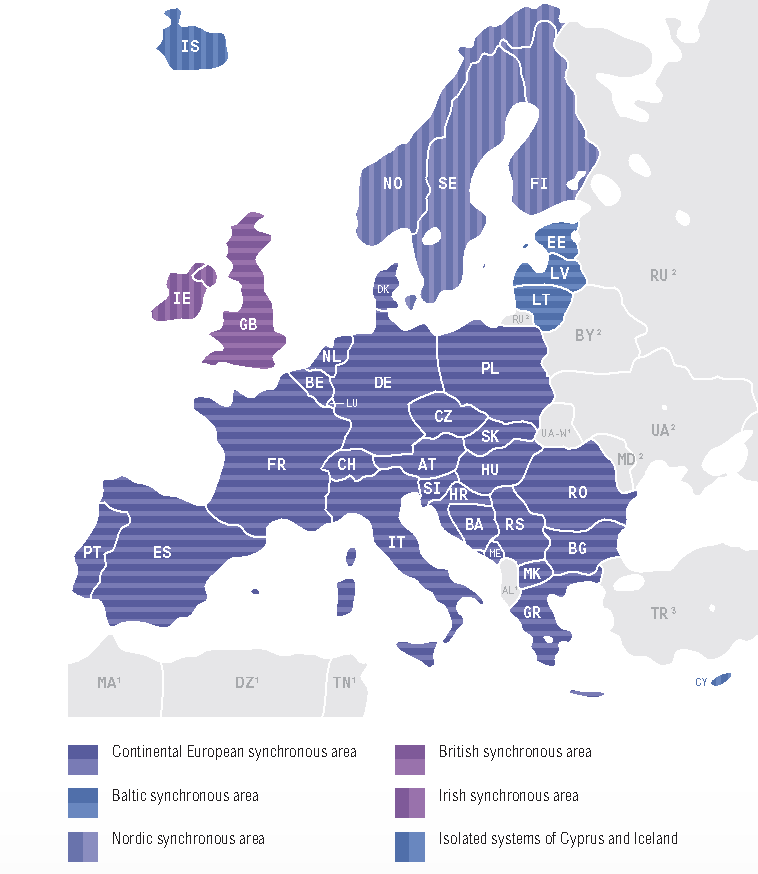
\includegraphics[height=13cm, width=14cm]{figures/ENTSO-E-member-states.png}
    \caption[size = 9]{Synchronous areas in Europa \cite{synchronous_regions}.}
    \label{fig:theory:entso-synchronous-area}
\end{figure}

The power producing units in a conventionally electric power system have typically consisted of spinning masses. The generators and turbines have a large masses and together give the power system an associated moment of inertia \textit{J}. The system inertia naturally gives frequency stability to the system. However, renewable energy sources do not have any natural inertia that helps the stability in frequency. Wind power have rotating masses, but they generally use asynchronous generators that do not follow the frequency of the grid SOURCE. Harnessing solar power by using photo voltaic (PV) modules does not involve physical inertia, and does therefore not contribute to frequency stability. A possible solution to this problem is to use virtual inertia on renewable power that mimics the reaction of a synchronous generator \cite{virtual_inertia}. From the transmission system operator's perspective, renewable energy sources can look as if they are synchronous generators.


\section{Active network management}
Active network management (ANM) is a control strategy too avoid that components in a network exceeds its safety margins in stressed situations \cite{active_network_management}. This is specially relevant with the rising installation of solar panels in private households and large wind farms. A transmission system is constructed to produce power at centralised power plants, and the goal of the transmission system operator is to transport this power through the network and to the consumers. However, the role of the consumer has changed with the rising use of solar panels in private households. In sunny days, households with solar panels will become producers of energy, and send a large amount of power to the grid. The transmission grid is evolving from a centralised to a distributed energy system, with many smaller production units. This is called distributed energy resources (DER) and offers new challenges in terms of overloads and congestion in the grid. 


\end{document}
